\subsection*{Effective thermal marginal}

Having established when the subsystem relaxes, we next ask what distribution the relaxed subsystem approaches.
The subsystem-relaxation measurements above show that, in the relaxed
regime defined by the memory order parameter, the measured subsystem
distribution becomes nearly independent of the initial subsystem state.
They do not by themselves determine whether the common distribution has a
thermal form.  We therefore compare the measured marginal $P_S$ with a
classical conditional Boltzmann marginal evaluated at an effective inverse
temperature calibrated on independent one-qubit probes.

\paragraph{In-situ $\beta_\mathrm{eff}$ calibration.}
Following the spirit of classical thermometry protocols for quantum
annealers~\cite{grattan2025thermometry}, we define $\beta_\mathrm{eff}$
operationally as the Boltzmann slope of the $z$-basis readout distribution
produced by the complete reverse-anneal protocol on a single-qubit probe.  We submit Ising problems consisting of
one active qubit with longitudinal bias $h=0.5$ and no couplings, use the
same reverse-anneal schedule as the many-body experiment
($s_p=0.4$, $t_p=100\,\mu$s, \texttt{auto\_scale=False}, 5{,}000 reads per
initial state), and estimate
\begin{equation}
    \beta_\mathrm{eff}
    = \frac{1}{2h}
      \ln\!\left(\frac{n_\downarrow}{n_\uparrow}\right),
    \label{eq:beta_eff}
\end{equation}
with the result averaged over three probe qubits drawn from the solver
nodelist.  For the main thermal-marginal sweep on Advantage2
(native exact-enumeration, random-regular exact-enumeration, Hamiltonian-scale, large-bath and disorder sub-experiments), taken after
the Advantage2 solver rename and recalibration, this procedure gives
$\beta_\mathrm{eff}=7.219\pm0.063$ at $s_p=0.4$; the frustrated pilot
described below was submitted in a separate run and uses an independently
recalibrated $\beta_\mathrm{eff}=7.331\pm0.198$.  For the
Advantage\_system6.4 cross-QPU replication the same procedure gives
$\beta_\mathrm{eff}=4.289\pm0.294$.  All three values should be
distinguished from the earlier main-experiment calibration of
$\beta_\mathrm{eff}=6.93\pm0.20$ (Advantage2) and
$4.46\pm0.26$ (Advantage\_system6.4) quoted elsewhere in the paper.  In
every case, $\beta_\mathrm{eff}$ is a protocol-level readout parameter:
it is not identified with the refrigerator temperature, nor with a
quantum Gibbs temperature of the pause-point Hamiltonian.

\paragraph{Conditional Gibbs prediction.}
For the thermal-marginal data analyzed here, the environment is prepared in
a fixed ordered state.  The corresponding classical target for the
subsystem is therefore the conditional marginal
\begin{equation}
    P_S^\mathrm{th}(\sigma_S \mid \sigma_E = \mathbf{1})
    =
    \frac{
        \exp[-\beta_\mathrm{eff}
        H_P(\sigma_S,\sigma_E=\mathbf{1})]
    }{
        \sum_{\sigma_S'}
        \exp[-\beta_\mathrm{eff}
        H_P(\sigma_S',\sigma_E=\mathbf{1})]
    },
    \label{eq:cond_gibbs}
\end{equation}
which we evaluate by direct enumeration of the $2^{|S|}$ subsystem
configurations with $\sigma_E$ held fixed.  This conditional object differs
from an unconditional equilibrium marginal, which averages over environment
configurations and therefore does not encode the prepared symmetry-breaking
boundary condition.  In globally spin-flip-symmetric instances, the
unconditional marginal would average over the two ordered sectors and
predict zero subsystem magnetization.

\paragraph{Main result.}
In a 10-seed disorder sweep at fixed $N=12$, $|S|=4$, $\lambda=0.5$ on a
3-regular logical graph (Fig.~\ref{fig:thermal_marginal}), the measured marginal agrees with the
conditional classical prediction whenever the memory criterion identifies
the instance as relaxed.  Over the tested values
$W\in\{0,0.25,0.5,0.75,1.0,1.25\}$, the mean
$D_\mathrm{TV}(P_S^\mathrm{exp},P_S^\mathrm{th})$ over relaxed disorder
realisations lies between
$0.6\times10^{-3}$ and $3.6\times10^{-3}$, below the estimated
multinomial sampling floor for this comparison and with no clear monotone
dependence on $W$ (Fig.~\ref{fig:thermal_marginal}b).  In the same sweep, the fraction of relaxed
disorder realisations decreases from $10/10$ at $W=0$ to $4/10$ at $W=1.25$
(Fig.~\ref{fig:thermal_marginal}a), consistent with the disorder-induced arrest reported above.
Thus, within this sweep, disorder primarily controls whether the subsystem
reaches the common marginal; conditioned on relaxation, the common marginal
is consistent with the calibrated conditional Boltzmann form.

The same diagnostic gives the same qualitative conclusion at the
main-experimental scale.  For $|S|=6$, $|E|=50$ on native Zephyr
subgraphs, $11/14$ conditions are relaxed across the two Hamiltonian
scales ($5/7$ unscaled and $6/7$ at scale $0.5$), and every one of
those $11$ relaxed conditions satisfies
$D_\mathrm{TV}<10^{-3}$ against the classical conditional target, with
maxima $5.0\times10^{-4}$ and $2.6\times10^{-4}$ in the two sets
respectively.  Across the full $494$-condition thermal-marginal sweep on
Advantage2 (native Zephyr, random 3-regular, three Hamiltonian scales,
large-bath native and disorder sub-experiments), $113/494$ conditions satisfy the relaxation
criterion, and all but three of them have classical conditional
$D_\mathrm{TV}$ below $0.05$; the three exceptions are the two severe
wrong-basin trapping instances and one borderline miss described below.
An independent $60$-condition cross-QPU replication on
Advantage\_system6.4 agrees qualitatively: $22/60$ instances satisfy
$\mathcal{M}\le0.05$ at the separately calibrated
$\beta_\mathrm{eff}=4.29$, with classical conditional $D_\mathrm{TV}$
distributed over $[3\times10^{-5},\,0.029]$ and median $0.005$.  These
passing conditions span graph geometry (random 3-regular and native
Zephyr), subsystem size ($|S|\in\{4,6\}$), coupling strength
($\lambda\in\{0.2,0.3,0.5\}$), and Hamiltonian energy scale (overall
factors $0.35$, $0.5$, $0.75$, and $1.0$).  The comparison therefore
provides a thermal-marginal test that is separate from, and stricter
than, loss of initial-state memory alone (Fig.~\ref{fig:thermal_marginal}c).

\paragraph{Quantum reduced Gibbs diagnostic.}
The same comparison can be repeated with the $z$-basis diagonal of the
quantum reduced Gibbs state of the pause-point Hamiltonian,
\begin{equation}
    H(s_p)
    =
    -\frac{A(s_p)}{2}\sum_i \sigma_x^i
    + \frac{B(s_p)}{2} H_P ,
    \label{eq:Hsp}
\end{equation}
evaluated on the full $N$-qubit system by exact diagonalisation for
$N\le12$, with the transverse field retained at $s_p$.  We use the same
protocol-level $\beta_\mathrm{eff}$ and the device-calibrated ratio
$A(s_p)/B(s_p)=0.260$ for Advantage2 and $0.259$ for
Advantage\_system6.4, extracted directly from the solver anneal-schedule
spreadsheets at $s_p=0.4$.  Two quantum targets are compared against the
pooled measured marginal: the \emph{conditional} quantum reduced Gibbs
marginal with $\sigma_E$ fixed to the prepared ordered state, and the
\emph{unconditional} marginal that traces over all $2^{|E|}$ environment
configurations.

The conditional quantum reduced Gibbs target is tight in the disorder
sweep but not uniformly across all scaled ferromagnetic
conditions.  On this disorder sweep at $N=12$, $|S|=4$, $\lambda=0.5$ on
a 3-regular logical graph, the median conditional quantum
$D_\mathrm{TV}$ across 43 relaxed Advantage2 conditions is $0.0145$
(max $0.0272$); on the 22 relaxed Advantage\_system6.4 conditions it is
$0.0146$ (max $0.0284$).  Across the 102 relaxed $N\le12$ ferromagnetic
main-sweep conditions for which the quantum target was computed,
$73$ satisfy $D_\mathrm{TV}\le0.05$ and $29$ exceed it, with the excesses
concentrated in the Hamiltonian-scale sweeps.  Scaling the problem
Hamiltonian by a factor $s$ leaves $A(s_p)$ unchanged but multiplies
$B(s_p)H_P$ by $s$, so the effective transverse-to-longitudinal ratio
seen by the reduced Gibbs state is $A/(sB)$; at scale $0.35$
this is $0.260/0.35\approx0.74$, at scale $0.5$ it is
$0.260/0.5\approx0.52$, and at scale $0.75$ it is
$0.260/0.75\approx0.35$.  The conditional quantum diagonal therefore
accumulates increasingly large transverse-field-induced excited-state
mixing at smaller scale, mixing that the measured post-return-ramp
readout does not display.  The unconditional quantum reduced Gibbs
marginal is a much worse target in every ferromagnetic regime (median
$D_\mathrm{TV}\approx 0.5$ in the Advantage2 disorder sweep), which is
expected because the unconditional marginal averages over both ordered
sectors of the global $Z_2$ and cannot encode the prepared all-up
boundary.

The residual gap between the classical and conditional quantum
predictions in the ferromagnetic regime is consistent with the
interpretation of the calibrated $\beta_\mathrm{eff}$ as a
protocol-level readout slope: the readout distribution is measured
after the return ramp to $s=1$, and the net protocol-level mapping
from the reverse anneal, pause, return ramp and readout absorbs the
small transverse-field-induced mixing that the conditional quantum
pause-point state would otherwise carry.  Within that single
$\beta_\mathrm{eff}$, both the classical and quantum conditional
predictions are consistent with the measurements, with the classical
conditional target the tighter of the two.

A frustrated pilot, in which the sign of each coupler is flipped with
probability $\tfrac12$ (Edwards--Anderson bond disorder) on top of the
random 3-regular $N=12$, $|S|=4$, $\lambda=0.5$ sweep at five disorder
seeds, inverts that ordering.  On the two conditions that satisfy
$\mathcal{M}\le0.05$, the classical conditional target has
$D_\mathrm{TV}=0.32$ on average (max $0.64$), while the conditional
quantum reduced Gibbs target has $D_\mathrm{TV}=0.029$ on average (max
$0.045$): an order-of-magnitude-tighter agreement in this small relaxed subset.
This pilot suggests that the frustrated regime can distinguish the two
predictions in the multi-modal classical-marginal regime, but a larger
frustrated campaign is needed to establish the effect.  The evidence
for quantum effects in the main paper continues to enter primarily
through the relaxation dynamics---including the $s_p$-dependent
relaxation trends and the failure of device-temperature Glauber
dynamics to reproduce the observed initial-state mixing.  In the
ferromagnetic regime, the final relaxed $z$-basis weights are
consistent with either reduced Gibbs target at the same
$\beta_\mathrm{eff}$; the frustrated pilot instead favours the
conditional quantum target by roughly an order of magnitude on its
two relaxed instances, but this subset is too small to establish the
effect and motivates a dedicated frustrated campaign.

\paragraph{Dynamical-trapping failure modes.}
Three relaxed conditions in the 494-instance thermal-marginal sweep fail
the thermal-marginal test against the classical conditional target at
$D_\mathrm{TV}>0.05$.  Two of them are severe wrong-basin failures
corresponding to the same physical instance, $\lambda=0.2$, $N=8$,
$W=1.0$, seed~42 on a native Zephyr subgraph, observed at two
Hamiltonian scales.  At scale $0.35$ the memory order parameter is
$\mathcal{M}=0.0145$, the classical conditional
$D_\mathrm{TV}(P_S^\mathrm{exp},P_S^\mathrm{th})=0.9409$, and the
conditional quantum reduced Gibbs $D_\mathrm{TV}=0.5414$; at scale $0.5$
the corresponding values are $\mathcal{M}=0.0240$,
$D_\mathrm{TV}(\mathrm{classical})=0.9674$, and
$D_\mathrm{TV}(\mathrm{quantum~cond.})=0.3565$.  A third relaxed
condition with the same $(\lambda,N,W)$ but seed~123 at scale $0.35$ is
a borderline miss rather than a wrong-basin trap
($\mathcal{M}=0.0085$, $D_\mathrm{TV}=0.0513$), with measured
magnetisation close to $+1$ on every subsystem site.

For the severe scale-$0.5$ trapping instance, the three initial
subsystem states converge to nearly the same measured distribution, but
that distribution places $98.5\%$ of its weight on the higher-energy
all-down basin rather than on the classical all-up ground state.  Direct
enumeration of the conditional classical energies in the scaled units
gives $E_\uparrow=-1.7142$ and $E_\downarrow=-1.1675$, so at
$\beta_\mathrm{eff}=7.219$ the classical Boltzmann weight favours the
all-up basin by
$\exp[\beta_\mathrm{eff}(E_\downarrow-E_\uparrow)]\approx 52$.  The
scale-$0.35$ twin shows the same all-down localisation with
$\mathcal{M}=0.0145$.

Both wrong-basin instances are therefore consistent with dynamical
trapping into a common non-thermal basin rather than with incomplete
relaxation: the memory order parameter is below the relaxation
threshold in each case, but the converged distribution does not match
either the classical conditional or the conditional quantum reduced
Gibbs target.  Reporting the memory order parameter and the
thermal-marginal distance as two independent quantities separates
ordinary relaxation from this failure mode, and identifies the same
trapping pair whether the thermal target is the classical conditional
or the conditional quantum reduced Gibbs marginal.

The same comparison also acts as a diagnostic outside the relaxed regime,
though low pooled $D_\mathrm{TV}$ is not equivalent to relaxation.
Among the $381$ memory-retaining thermal-marginal conditions with $\mathcal{M}>0.05$,
the classical conditional distance against the prepared-$E$ target
spans $[0.003, 0.97]$ with median $0.35$; larger memory is generally
accompanied by larger deviation from the conditional Gibbs prediction,
but $22/381$ memory-retaining conditions have $D_\mathrm{TV}<0.05$
because the three-initial-state pooled marginal can accidentally
resemble the conditional target even when the individual initial-state
distributions remain distinct.  Reporting $\mathcal{M}$ and
$D_\mathrm{TV}$ together therefore separates ordinary relaxation to the
thermal marginal, the small number of relaxed-but-non-thermal trapping
instances, and these memory-retaining accidental-pool matches, and the
classification is stable under the corrected device-calibrated
$A(s_p)/B(s_p)$.

\begin{figure*}[!htbp]
\centering
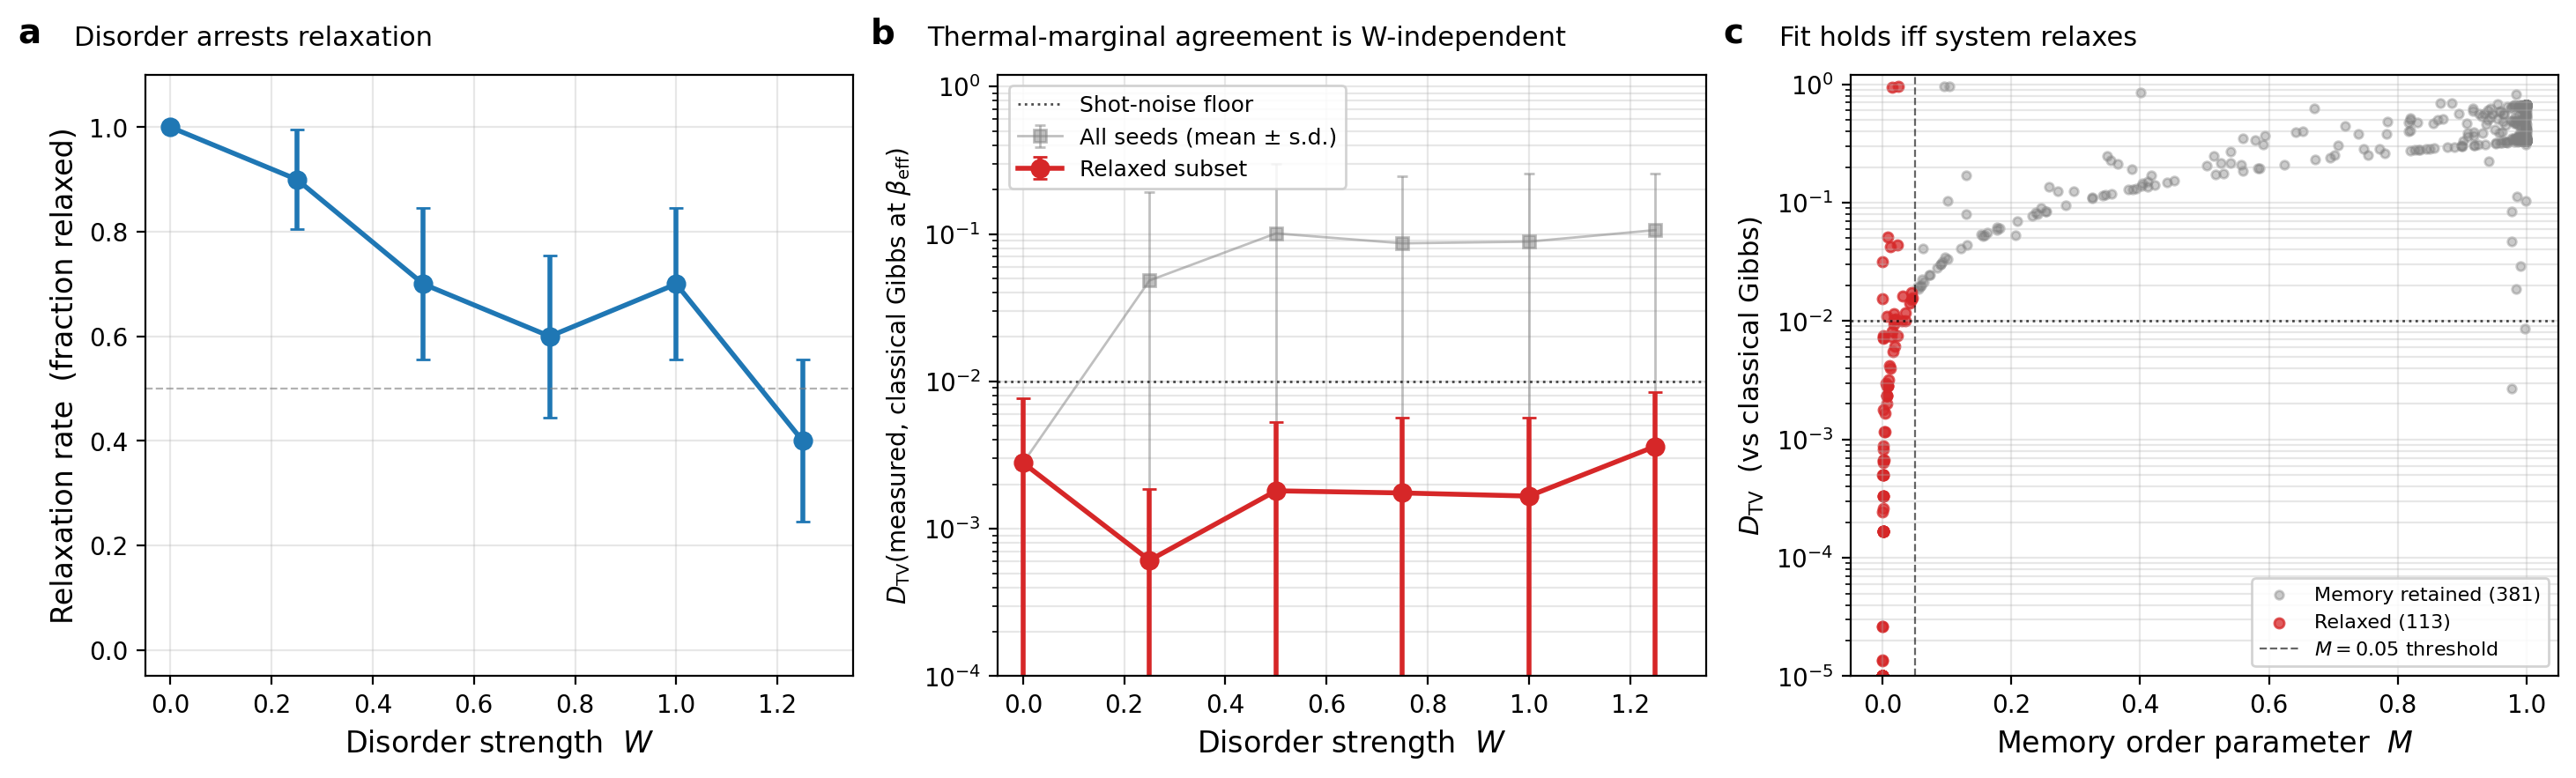
\includegraphics[width=\textwidth,height=0.72\textheight,keepaspectratio]{figures/fig6_thermal_marginal.pdf}
\caption{\textbf{Effective thermal marginal.}
\textbf{a,}~Fraction of relaxed disorder realisations ($\mathcal{M}\le 0.05$) in the 10-seed disorder sweep ($N=12$, $|S|=4$, $\lambda=0.5$, 3-regular logical graph, Advantage2).  Relaxation fraction decreases from $10/10$ at $W=0$ to $4/10$ at $W=1.25$.
\textbf{b,}~Total-variation distance between the pooled subsystem marginal and the calibrated classical conditional Gibbs target at $\beta_\mathrm{eff}=7.219$ vs disorder strength.  Open circles: all 10 seeds; filled circles: relaxed subset only (error bars = s.d. across relaxed seeds).  Grey band: finite-shot reference $D_\mathrm{TV}\simeq\tfrac12\sqrt{K/N_\mathrm{reads}}\approx 0.026$ with $N_\mathrm{reads}=6000$, $K=2^{|S|}=16$; the relaxed subset stays at or below this scale across the sweep.
\textbf{c,}~Scatter of $D_\mathrm{TV}$ vs $\mathcal{M}$ across all thermal-marginal conditions.  Red: relaxed ($\mathcal{M}\le 0.05$); grey: memory-retaining.  Two top-left red outliers correspond to the same $\lambda=0.2$, $N=8$, $W=1$, seed~42 native Zephyr instance at Hamiltonian scales $0.35$ and $0.5$ (dynamical trapping, discussed in the body).  The memory and thermal-marginal criteria identify the same condition set apart from this trapping pair and one borderline $D_\mathrm{TV}=0.051$ miss.}
\label{fig:thermal_marginal}
\end{figure*}
